\documentclass[a4paper]{article}

\usepackage[utf8]{inputenc}
\usepackage[brazil]{babel}
\usepackage{graphicx}

\usepackage{natbib}

\title{Aula latex}
\author{Fernando Mayer}
\date{\today}

\begin{document}

\maketitle
\tableofcontents

\section{Introdução}

O LaTeX é um conjunto de {\bf macros} para o processador de textos TeX, utilizado amplamente para a produção de \textbf{textos matemáticos} e \textit{científicos} devido à sua alta qualidade tipográfica. Entretanto, também é utilizado para produção
de cartas pessoais, artigos e {\Large livros} sobre assuntos diversos.

Nova parágrafo.

E outro.

\begin{center}
Texto centralizado.
\end{center}

O Word não possui nem $\sim$ 10\% da capacidade de editoração do LaTeX!

\section{Metodologia}

\subsection{Dados}

Os dados foram coletados da seguinte forma:

\begin{itemize}
\item Forma 1
\item Forma 2
\end{itemize}

Os dados foram importados com:

\begin{verbatim}
dados <- read.table("pib_gapminder.csv", header = TRUE,
                    sep = ",", dec = ".")
\end{verbatim}

\subsection{Análise}

As análises foram:

\begin{enumerate}
\item Análise 1
\begin{enumerate}
\item Sub analise 1
\item Sub analise 2
\end{enumerate}
\item Análise 2
\end{enumerate}

\section{Resultados}

A relação entre expvida e pibpercap pode ser vista na figura \ref{fig:plot}.

\begin{figure}[h]
\centering
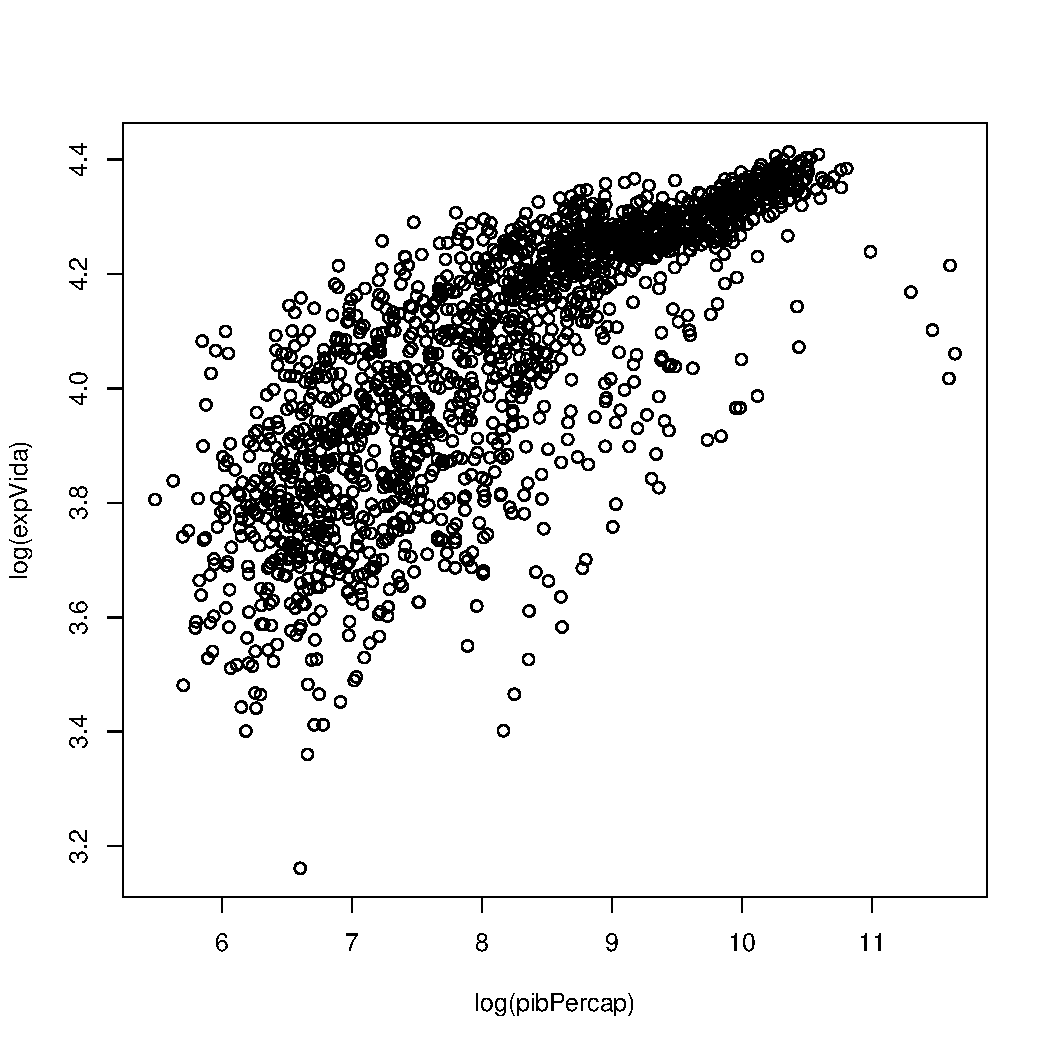
\includegraphics[width=0.8\textwidth]{figura1.pdf}
\caption{Legenda da figura.}
\label{fig:plot}
\end{figure}

\section{Discussão}

Veja a tabela \ref{tab:medias}.

\begin{table}[h]
\caption{Média de expVida por continente.}
\label{tab:medias}
\centering
\begin{tabular}{cc}
\hline
Continente & expVida \\
\hline
Africa & 48.87 \\
Americas & 64.66 \\
Asia & 60.07 \\
Europe & 71.90 \\
Oceania & 74.32 \\
\hline
\end{tabular}
\end{table}

Uma equação $a+b-2c$ e outra

\begin{equation}
\label{eq:a}
a+b-2c
\end{equation}

Veja a equação \ref{eq:a}.

A densidade da normal é

\begin{equation}
f(x) = \frac{1}{\sigma \sqrt{2\pi}} \exp{ \left[ -\frac{1}{2}
    \left( \frac{x - \mu}{\sigma} \right)^2 \right] }
\end{equation}


Segundo \citet{Buckland2004} dsdsds. E outra coisa \citep{Durbin1997}.

\bibliographystyle{apa}
\bibliography{ref}


\end{document}
